\documentclass[twoside, 10pt]{article}

% Русский перевод статьи noether_casimir_drive.tex (рабочий вариант для осмысления).
% Оригинал для подачи — noether_casimir_drive.tex (английский).

\usepackage[T1, T2A]{fontenc}   % Standard package for selecting font encodings
\usepackage[utf8]{inputenc} % Accept different input encodings
\usepackage[english, ukrainian, russian]{babel}

\usepackage{mathptmx}

\usepackage{indentfirst}    % Indent first paragraph after section header

\usepackage{sectsty}        % Control sectional headers

\sectionfont{\normalfont\Large\textbf}
\subsectionfont{\normalfont\large\textbf}

\usepackage{multicol}       % Intermix single and multiple columns
\usepackage{orcidlink}      % Insert hyperlinked ORCiD logo
\usepackage{fancyhdr}       % Extensive control of page headers and footers

\usepackage{filecontents}
\usepackage{hyperref, doi}
\usepackage[numbers]{natbib}

\bibliographystyle{myunsrtnat}

% --- METADATA ---
\def\myfirstpage{1}
\def\mylastpage{15}
\def\mypages{\myfirstpage-\mylastpage}
\def\myfilename{noether_casimir_drive_ru_v2}
\def\myname{А. Дроздов}
\def\mynameukr{А. Дроздов}
\def\mytitle{Теорема Нётер и сотовый двигатель Казимира: о несохранении импульса в асимметричных вакуумных системах}
\def\mytitleukr{Теорема Нетер та стільниковий рушій Казимира: про незбереження імпульсу в асиметричних вакуумних системах}
\def\myissn{2222-5617}
\def\mydoi{10.26565/2222-5617-2026-XX-XX} % ← placeholder, замените при подаче
\def\myemail{alexey.drozdov.07@gmail.com}
\def\ukrvisnyk{Вісник Харківського національного університету імені В.~Н.~Каразіна, серія «Фізика», вип. XX, \mypages~(2026)}
\def\ruvisnyk{Вестник Харьковского национального университета имени В.~Н.~Каразина, серия «Физика», вып. XX, \mypages~(2026)}
\def\myworkplace{Харьковский национальный университет имени В.~Н.~Каразина, пл. Свободы, 4, 61022 Харьков, Украина}
\def\myworkplaceukr{Харківський національний університет імені В.~Н.~Каразіна, майдан Свободи, 4, 61022 Харків, Україна}
\def\mynameen{A. Drozdov}
\def\mytitleen{Noether's theorem and the Casimir honeycomb drive: on non-conservation of momentum in asymmetric vacuum systems}
\def\myworkplaceen{V.~N.~Karazin Kharkiv National University, 61022, 4 Svoboda Sq., Kharkiv, Ukraine}
\def\myreceiveden{Received on January 9, 2026.}
\def\myaccepteden{Accepted for publication on January 9, 2026.}
\def\myorcidlink{0009-0004-1386-4534}

\def\myreceived{Поступила в редакцию 9 января 2026 г.}
\def\myaccepted{Принята к печати 9 января 2026 г.}
\def\myreceivedukr{Надійшла до редакції 9 січня 2026 р.}
\def\myacceptedukr{Прийнято до друку 9 січня 2026 р.}

\def\licenseref{http://creativecommons.org/licenses/by/4.0/}

\def\myvspacebeforesubsection{-2.0mm}
\def\myvspaceaftersubsection{-2.5mm}

\def\collontitulasfontcode{lmss}

\newcommand{\MyTitle}{\expandafter\MakeUppercase\expandafter{\mytitle}}
\newcommand{\MyTitleUkr}{\expandafter\MakeUppercase\expandafter{\mytitleukr}}

\fancypagestyle{firstpagestyle}{
\renewcommand{\headrulewidth}{0.6pt}
\fancyhead[C]{\ukrvisnyk \\ \ruvisnyk}
\renewcommand{\footrulewidth}{0.6pt}
\fancyfoot[L]{\footbox{${}^{\copyright}$ \myname}}
\fancyfoot[R]{\footbox[r]{\fontencoding{T1}\fontfamily{\collontitulasfontcode}\selectfont \textit{Open Access. This article is licensed under a Creative Commons Attribution 4.0} \\
\href{\licenseref}{\textit{\licenseref}}}}
}

\usepackage{graphicx}
\usepackage{caption}
\DeclareCaptionFormat{nocaption}{}
\captionsetup{format=nocaption,aboveskip=0pt,belowskip=0pt}
\usepackage{float}
\floatplacement{figure}{H}
\usepackage{xcolor}
\usepackage{enumerate}
\usepackage{geometry}
\usepackage{amsmath, amssymb}
\usepackage{textcomp}
\usepackage{upquote}
\usepackage{ucs}
\usepackage{grffile}
\usepackage[Export]{adjustbox}
\adjustboxset{max size={0.9\linewidth}{0.9\paperheight}}
\usepackage{longtable, booktabs, enumitem, ulem, wrapfig, sidecap}

\providecommand{\keywords}[1]{\textbf{\textit{Ключевые слова:}} #1}
\providecommand{\keywordsukr}[1]{\textbf{Ключові слова:} #1}

\author{\myname \,\orcidlink{\myorcidlink}}
\title{\textbf{\MyTitle.}}
\date{}

\definecolor{urlcolor}{rgb}{0,.145,.698}
\definecolor{linkcolor}{rgb}{0,0,0}
\definecolor{citecolor}{rgb}{0,0,0}

\providecommand{\doi}[1]{DOI: \href{https://doi.org/#1}{#1}}

\geometry{verbose,a4paper,includehead,includefoot,
nomarginpar,
headheight=26pt,footskip=58pt,
tmargin=1.1cm,bmargin=1.0cm,lmargin=1.85cm,rmargin=1.85cm}
% Многострочные колонтитулы: \footbox выравнивает блок по нижней строке, поэтому он растёт
% вверх от базовой линии footskip и не уходит за край листа; footskip (58pt) больше высоты
% четырёх строк \scriptsize, поэтому текст на колонтитул не наезжает.
\newcommand{\footbox}[2][l]{\parbox[b]{0.88\linewidth}{\scriptsize\if#1r\raggedleft\else\raggedright\fi #2}}

\setlength{\columnsep}{0.5cm}

% forbid word transfer
\hyphenpenalty=10000

\begin{document}

\fontencoding{T2A}\fontfamily{ptm}\selectfont

\setcounter{page}{\myfirstpage}

\pagestyle{fancy}
\fancyhead{}
\fancyhead[CE]{\fontencoding{T2A}\fontfamily{ptm}{\selectfont \textit{\mytitle.}}}
\fancyhead[CO]{\fontencoding{T2A}\fontfamily{ptm}{\selectfont \textit{\myname}}}
\renewcommand{\headrulewidth}{0.6pt}
\fancyfoot{}
\fancyfoot[LE,RO]{\thepage}
\fancyfoot[LO]{\footbox{{\fontencoding{T2A}\fontfamily{ptm}\selectfont \ruvisnyk} \\ {\fontencoding{T2A}\fontfamily{\collontitulasfontcode}\selectfont \ukrvisnyk}}}
\fancyfoot[RE]{\footbox[r]{{\fontencoding{T2A}\fontfamily{ptm}\selectfont \ruvisnyk} \\ {\fontencoding{T2A}\fontfamily{\collontitulasfontcode}\selectfont \ukrvisnyk}}}
\fancyfoot[CO,CE]{}

$\,$

\thispagestyle{firstpagestyle}

\vspace{-9.4mm}

\begin{tabular}{lcr}
\doi{\mydoi}
& \,\,\,\,\,\,\,\,\,\,\,\,\,\, \,\,\,\,\,\,\,\,\,\,\,\,\,\, \,\,\,\,\,\,\,\,\,\,\,\,\,\, \,\,\,\,\,\,\,\,\,\,\,\,\,\, \,\,\,\,\,\,\,\,\,\,\,\,\,\, \,\,\,\,\,\,\,\,\,\,\,\,\,\,
& ISSN \myissn (Print)
\end{tabular}

\vspace{9mm}

\begin{tabular}{l}
Оригинальная статья \\
Статья в печати \\
\href{https://doi.org/\mydoi}{https://doi.org/\mydoi} \\
УДК 53.09, 621.3, 629.7 \\
PACS: 11.10.Ef, 03.70.+k, 42.50.Lc \\
\end{tabular}

\section*{\centering {\fontencoding{T2A}\fontfamily{ptm}{\selectfont \MyTitle}}}

\vspace{7mm}
\centerline{\Large{\myname \,\orcidlink{\myorcidlink} }}
\vspace{7.5mm}
\centerline{\textit{\myworkplace}}
\centerline{\textit{E-mail: \href{mailto:\myemail}{\myemail}}}

\vspace{5mm}
\centerline{\myreceived}
\centerline{\myaccepted}

\vspace{5mm}

В работе сотовый двигатель Казимира \cite{Drozdov2024} --- идеально проводящая пластина
с нанорозмерной сотовой структурой на одной стороне --- рассматривается с точки зрения симметрий.
Из-за асимметрии вакуумных мод по разные стороны пластины система не инвариантна относительно
трансляций вдоль нормали: вакуумный гамильтониан явно зависит от координаты \(l\), и по теореме
Нётер импульс поля вдоль этой оси не сохраняется. Сила тяги равна \(\partial\langle H\rangle/\partial l\).
Затем та же сила вычислена независимо --- через тензор натяжений Максвелла, построенный из полей
собственных мод резонатора. Помодово оба вывода совпадают тождественно (теорема Гельмана--Фейнмана),
а после регуляризации совпадают в пределе \(ak_m\to\infty\). Попутно найдена и исправлена ошибка
в приложении~B работы \cite{Drozdov2024}: для TM-мод отношение давления к плотности энергии равно
\(k_z^2/k^2\), а не единице. Тензорный расчёт показывает, где приложена сила: это скачок
\(\langle T_{zz}\rangle\) на поверхности металла, и поэтому поток импульса через любую замкнутую
вакуумную поверхность, охватывающую пластину, не зависит от положения её граней. Наконец, показано,
что стандартный баланс импульса (\S\,105 Тамма) при \(\langle\mathbf S\rangle=0\) теряет именно
эти скачковые члены. Не сохраняется импульс поля (и пластины); полный импульс системы
\emph{пластина\,+\,поле\,+\,опора} сохраняется.

\vspace{5mm}

\noindent
\begin{keywords}
\textit{теорема Нётер, эффект Казимира, квантовый вакуум, несохранение импульса, наносоты, тяга Казимира}
\end{keywords}

\vspace{5mm}

\noindent
\textbf{Як цитувати}: \textit{\mynameukr}. \textit{\mytitleukr}. {\ukrvisnyk}. \href{https://doi.org/\mydoi} {https://doi.org/\mydoi}.

\vspace{5mm}

\noindent
\textbf{Как цитировать}: \textit{\myname}. \textit{\mytitle}. {\ruvisnyk}. \href{https://doi.org/\mydoi} {https://doi.org/\mydoi}.

\vspace{5mm}

\newpage

\begin{multicols}{2}

\vspace{\myvspacebeforesubsection}
\subsection*{\centering{\fontencoding{T2A}\fontfamily{ptm}{\selectfont ВВЕДЕНИЕ}}}
\vspace{\myvspaceaftersubsection}


В работе \cite{Drozdov2024} было показано, что идеально проводящая пластина, одна сторона
которой гладкая, а другая покрыта сотами с квадратной ячейкой \(a\times a\), испытывает со
стороны электромагнитного вакуума результирующую силу. Сила вычислялась как разность плотностей
энергии нулевых колебаний по обе стороны пластины, регуляризованная по формуле
Эйлера--Маклорена; для ячейки \(a\approx2\)~мкм она оказалась порядка нескольких дин на
квадратный метр.

Такой результат неизбежно вызывает вопрос: как однотельная сила совместима с сохранением
импульса? В классической конфигурации Казимира с двумя пластинами силы, действующие на пластины,
равны и противоположны, и вопрос не возникает. Здесь второго тела нет.

Настоящая работа отвечает на этот вопрос в три шага.

\textit{Первый шаг --- симметрия.} Теорема Нётер \cite{Noether1918} связывает сохранение
импульса с трансляционной инвариантностью. Сотовая пластина эту инвариантность нарушает, поэтому
импульс поля сохраняться не обязан, а сила равна производной вакуумного гамильтониана по
положению пластины. Этот результат совпадает с силой из \cite{Drozdov2024}.

\textit{Второй шаг --- независимая проверка.} Если сила реальна, её должен давать и тензор
натяжений Максвелла. Мы строим его непосредственно из полей собственных мод резонатора и
показываем, что для каждой моды тензорный и гамильтонов выводы совпадают. Эта проверка выявила
ошибку в приложении~B работы \cite{Drozdov2024}, которую мы исправляем; на гамильтонов результат
она не влияет.

\textit{Третий шаг --- где сила приложена и куда уходит импульс.} Тензорный расчёт показывает, что
сила сосредоточена в скачке тензора натяжений на поверхности металла. Стандартное уравнение
баланса импульса (\S\,105 Тамма \cite{Tamm1957}) этих скачков не содержит; при нулевом среднем
векторе Пойнтинга это и создаёт видимость парадокса. Мы указываем недостающий член и
формулируем, какой именно импульс не сохраняется.

Все численные утверждения статьи проверены в сопровождающем Jupyter-ноутбуке \cite{VerifNotebook}.

\vspace{\myvspacebeforesubsection}
\subsection*{\centering{\fontencoding{T2A}\fontfamily{ptm}{\selectfont ПОСТАНОВКА ЗАДАЧИ}}}
\vspace{\myvspaceaftersubsection}


Пластина нулевой толщины лежит в плоскости \(z=0\) внутри куба \(L^3\) с идеально проводящими
стенками (рис.~1). Со стороны \(z>0\) на пластине стоят идеально проводящие ячейки сечения
\(a\times a\), стенки которых доходят до грани куба \(z=l\) (в \cite{Drozdov2024} \(l=L/2\)).
Со стороны \(z<0\) находится гладкая сторона пластины и большая полость
\(L\times L\times(L-l)\).

Каждая полость есть прямоугольный резонатор \(a\times b\times h\): для ячейки \(a=b\), \(h=l\);
для большой полости \(a=b=L\), \(h=L-l\). Волновые числа
\(k_x=\pi n_x/a\), \(k_y=\pi n_y/b\), \(k_z=\pi n_z/h\); \(K^2=k_x^2+k_y^2\), \(k^2=K^2+k_z^2\),
\(\omega=ck\). Запись \(\sum_{n=(0)1}^{\infty}\) означает, что слагаемые с \(n=0\) входят с
весом \(\tfrac12\): каждому набору \((n_x,n_y,n_z)\) отвечают две поляризации, а при одном нулевом
индексе --- только одна \cite{Drozdov2024}.

\begin{figure}
\begin{center}
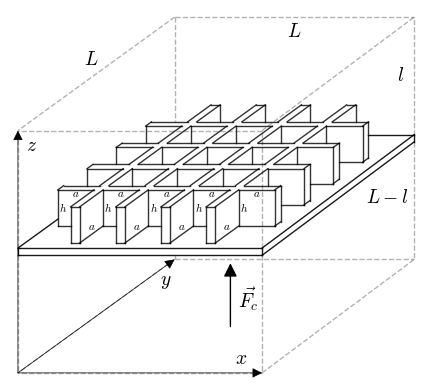
\includegraphics[width=0.42\textwidth]{honeycomb_box_H.png}
\caption{}{\centering{\textbf{Рис.1.} Кубический резонатор с пластиной, покрытой сотами.}}
\end{center}
\label{fig:honeycomb_box_H}
\end{figure}

Идеально проводящие стенки куба, как и у Казимира, --- вспомогательное граничное условие без
физического прообраза, подобное периодическим граничным условиям, которыми в учебниках квантовой
механики нормируют плоские волны. Процедура законна потому, что результат берётся в пределе
\(L\to\infty\): по теореме Вейля \cite{Weyl1912} главный член числа мод, \(N(k)\simeq Vk^3/3\pi^2\),
не зависит от граничных условий на внешних гранях, от них зависят лишь поверхностные поправки, и
вклад удалённых стенок в силу на пластину исчезает. Обрезание \(k_m\) --- отдельный, физический
элемент: его задаёт прозрачность материала пластины для коротких волн.

\vspace{\myvspacebeforesubsection}
\subsection*{\centering{\fontencoding{T2A}\fontfamily{ptm}{\selectfont ТЕОРЕМА НЁТЕР И НЕСОХРАНЕНИЕ ИМПУЛЬСА}}}
\vspace{\myvspaceaftersubsection}


Сумма энергий нулевых колебаний \(E=\frac12\sum\hbar\omega\) по обеим полостям даёт вакуумный
гамильтониан на единицу площади \cite{Drozdov2024}:

\end{multicols}

\[
\frac{\langle 0|\hat{\mathcal{H}}|0\rangle}{S} = \frac{\hbar c}{a^2\pi} \Bigg\{
l \sum_{n_x=(0)1}^{\infty}\sum_{n_y=(0)1}^{\infty}
\int_0^{\infty} \sqrt{ \frac{\pi^2}{a^2}(n_x^2 + n_y^2) + k_z^2 } \, dk_z
+ (L - l) \int_0^{\infty}\!\!\int_0^{\infty}
\int_0^{\infty} \sqrt{k_x^2 + k_y^2 + k_z^2} \, dk_z \, \frac{a}{\pi}dk_x \frac{a}{\pi}dk_y
\Bigg\}.
\]

\begin{multicols}{2}

Это выражение явно зависит от \(l\). Следовательно, система \textbf{не инвариантна} относительно
бесконечно малых трансляций пластины \(z\to z+\delta z\).

По теореме Нётер генератор пространственных трансляций --- компонента импульса \(P_z\) ---
сохраняется \textbf{тогда и только тогда}, когда гамильтониан не зависит от \(z\). Поскольку
\(\partial\langle H\rangle/\partial l\neq0\), симметрия нарушена, и \(P_z\) поля не сохраняется.
Результирующая сила равна

\end{multicols}

\[
\frac{F}{S} = \frac{\partial}{\partial l} \frac{\langle 0|\hat{\mathcal{H}}|0\rangle}{S}
= \frac{\hbar c}{a^2\pi} \left\{
\sum_{n_x=(0)1}^{\infty}\sum_{n_y=(0)1}^{\infty}
\int_0^{\infty} \sqrt{ \frac{\pi^2}{a^2}(n_x^2 + n_y^2) + k_z^2 } \, dk_z
- \int_0^{\infty}\!\!\int_0^{\infty}
\int_0^{\infty} \sqrt{k_x^2 + k_y^2 + k_z^2} \, dk_z \, dn_x dn_y
\right\},
\]

\begin{multicols}{2}

что совпадает с формулой тяги, полученной в \cite{Drozdov2024} через разность плотностей энергии.
После регуляризации \(f(k/k_m)\) и двумерного суммирования Эйлера--Маклорена она принимает вид
\(F/S=\delta(E/V)=R(ak_m)\,\hbar c\,\pi/a^4\).

Таким образом, появление тяги не является неожиданным: это прямое следствие нарушенной
трансляционной симметрии. Квантовый вакуум «давит» сильнее с одной стороны, потому что спектр
мод по сторонам пластины различен. Сразу оговорим, о каком импульсе идёт речь: нарушена
трансляционная симметрия \emph{граничных условий}, а не пространства. Поэтому не сохраняется
импульс поля --- или, что то же, пластины, которая его поглощает; полный импульс системы
\emph{пластина\,+\,поле\,+\,опора} сохраняется, как у обычного паруса на ветру. Где именно
поле передаёт импульс пластине, покажет тензор натяжений.

\vspace{\myvspacebeforesubsection}
\subsection*{\centering{\fontencoding{T2A}\fontfamily{ptm}{\selectfont ТЕНЗОР НАТЯЖЕНИЙ ИЗ ПОЛЕЙ МОД}}}
\vspace{\myvspaceaftersubsection}


Вычислим силу независимо, через тензор натяжений Максвелла, не предполагая заранее потока
импульса плоской волны. Явные поля TM- и TE-мод и проверка уравнений Максвелла и граничных
условий вынесены в приложение~А. Единицы гауссовы, обозначения Тамма \cite{Tamm1957}:
\(T_{ik}=\frac1{4\pi}(E_iE_k+H_iH_k)-\frac{\delta_{ik}}{8\pi}(E^2+H^2)\), сила на тела внутри
замкнутой поверхности равна \(\oint T_{ik}n_k\,dS\), поток импульса \(\Pi_{ik}=-T_{ik}\). Нам нужна
компонента
\[
T_{zz}=\frac1{8\pi}\left(E_z^2+H_z^2-E_x^2-E_y^2-H_x^2-H_y^2\right),
\]
давление на горизонтальную площадку обозначим \(p\equiv-\langle T_{zz}\rangle\).

\textbf{Давление одной моды.} Усредним \(T_{zz}\) по сечению \(ab\) и по периоду. При
\(n_x,n_y\ge1\) каждый множитель \(\sin^2\) или \(\cos^2\) даёт \(\tfrac12\), и для TM-моды
\[
8\pi\langle T_{zz}\rangle=\frac{A^2}{8}\left[\cos^2k_zz\left(1-\frac{k^2}{K^2}\right)-\frac{k_z^2}{K^2}\sin^2k_zz\right]
=-\frac{A^2}{8}\frac{k_z^2}{K^2},
\]
поскольку \(1-k^2/K^2=-k_z^2/K^2\). Плотность энергии той же моды, усреднённая по объёму,
\(8\pi\overline w=\frac{A^2}{8}\frac{k^2}{K^2}\). Следовательно,
\[
p=-\langle T_{zz}\rangle=\overline w\,\frac{k_z^2}{k^2}.
\]
Для TE-моды те же шаги дают тот же результат. Если один из поперечных индексов равен нулю (это
возможно только для TE), общий множитель удваивается и в давлении, и в энергии, отношение не
меняется; TM-мода с \(n_z=0\) имеет \(k_z=0\) и давления не создаёт.

\textbf{Независимость от \(z\).} Зависимость от \(z\) выпала (\(\cos^2+\sin^2=1\)). Общая причина:
в вакууме \(\partial T_{zk}/\partial x_k=\frac1{4\pi c}\,\partial_t[\mathbf E\times\mathbf H]_z\),
а среднее по периоду от производной по времени равно нулю. При интегрировании по сечению остаются
потоки через боковые стенки \(T_{zx}=\frac1{4\pi}(E_zE_x+H_zH_x)\); на стенках \(x=0,a\)
\(E_z=0\) (касательное поле) и \(H_x=0\) (нормальное), то есть \(T_{zx}=0\), и так же
\(T_{zy}=0\) на \(y=0,b\). Поэтому \(\frac{d}{dz}\int\langle T_{zz}\rangle\,dx\,dy=0\). Отметим:
от \(z\) не зависит только интеграл по сечению; в отдельной точке \((x,y)\) величина \(T_{zz}\)
меняется с \(z\), но в силу входит именно интеграл. Этот факт будет использован в следующем
разделе.

\textbf{Сумма по нулевым колебаниям.} Каждая мода есть осциллятор с энергией \(\hbar\omega/2\) в
основном состоянии, поровну распределённой между электрической и магнитной частями --- то же
распределение, что даёт классическое усреднение по периоду, если положить
\(\overline w\,V=\hbar\omega/2\). Поэтому давление в полости
\[
p=\frac{\hbar c}{2V}\sum_{\text{моды}}\frac{k_z^2}{k}.
\]
От суммы для энергии \(E=\frac{\hbar c}{2}\sum k\) она отличается только слагаемым: \(k_z^2/k\)
вместо \(k\).

\textbf{Тождество с гамильтоновым подходом.} При \(k_z=\pi n_z/h\) имеем
\(\partial k/\partial h=-k_z^2/(kh)\), и для каждой моды
\[
-\frac{\partial}{\partial h}\frac{\hbar ck}{2}=\frac{\hbar c}{2h}\frac{k_z^2}{k}=S\,p_{\text{моды}},\qquad V=Sh .
\]
Сила, найденная через тензор натяжений, совпадает с \(-\partial E/\partial h\) помодово, ещё до
какой-либо регуляризации (теорема Гельмана--Фейнмана \cite{Feynman1939}; иначе говоря,
сохранение адиабатического инварианта \(E/\omega\) каждой моды при медленном сдвиге стенки).
Тем самым гамильтонова сила предыдущего раздела подтверждена независимым методом.

\textbf{Исправление приложения~B работы \cite{Drozdov2024}.} Там давление на грань \(xy\)
вычислялось как \(\langle H_x^2+H_y^2\rangle/8\pi\). Для TM-мод при этом пропущен член
\(-\langle E_z^2\rangle/8\pi\): с ним отношение давления к плотности энергии равно \(k_z^2/k^2\)
для мод обоих типов, а не \(1\) для электрической моды (для моды \((2,1,3)\) при
\(a:b:h=1:1{,}3:2{,}7\) --- \(0{,}2119\) вместо \(1\)). Поэтому значение \(1\) для электрической
моды и опирающееся на него неравенство \(F/S\ge\delta(E/V)\) из \cite{Drozdov2024} неверны.
Гамильтонов вывод приложения~C при этом не затрагивается: по доказанному тождеству он помодово
совпадает с тензорным.

\textbf{Регуляризация.} С обрезанием \(f(k/k_m)\) производная энергии моды равна
\(-\partial_h\!\left[\frac{\hbar ck}{2}f\right]=\frac{\hbar c}{2h}\frac{k_z^2}{k}\left[f+\frac{k}{k_m}f'\right]\),
а регуляризованная тензорная сумма \(\sum(k_z^2/k)f\) второго члена не содержит. При конечном
\(ak_m\) два выражения поэтому различаются, но при \(ak_m\to\infty\) различие исчезает. Для
сотовой пластины это проверено численно (раздел «Проверки и оценки»).

\textbf{Симметрийная проверка.} Перенормированный тензор \(\langle T_{\mu\nu}\rangle\)
электромагнитного поля бесследов. Между двумя параллельными пластинами граничные условия
инвариантны относительно бустов вдоль пластин; вместе с условием на след это даёт
\(\langle\Pi_{zz}\rangle=3\langle u\rangle\) (Браун и Маклей \cite{BrownMaclay1969}). Ячейка сот ---
волновод вдоль \(z\): вдали от торцов её граничные условия инвариантны относительно бустов вдоль
\(z\), поэтому в блоке \((t,z)\) \(\langle T_{\mu\nu}\rangle\propto\eta_{\mu\nu}\) и
\(\langle\Pi_{zz}\rangle=-\langle u\rangle\), то есть \(|F/S|=\delta(E/V)\) --- то же значение,
что даёт гамильтонов подход. Аргумент точен для идеального проводника в пределе \(ak_m\to\infty\)
и с точностью до торцевых поправок порядка \(a/l\).

\vspace{\myvspacebeforesubsection}
\subsection*{\centering{\fontencoding{T2A}\fontfamily{ptm}{\selectfont ГДЕ ПРИЛОЖЕНА СИЛА}}}
\vspace{\myvspaceaftersubsection}


\textbf{Скачок на поверхности металла.} На грани \(z=0\) (вакуум снаружи, внутри металла поля
равны нулю) со стороны вакуума \(E_x=E_y=0\), \(H_z=0\), тогда как нормальное \(\mathbf E\) и
касательное \(\mathbf H\) испытывают скачки \(4\pi\sigma\) и \(\frac{4\pi}{c}\mathbf i\). Поэтому
\[
T_{zz}\big|_{\text{вакуум}}=\frac1{8\pi}\left(E_z^2-H_x^2-H_y^2\right),\qquad
T_{zz}\big|_{\text{металл}}=0 .
\]
Для TM-моды при \(z=0\) \(\langle E_z^2\rangle=\frac{A^2}{8}\),
\(\langle H_x^2+H_y^2\rangle=\frac{A^2}{8}\frac{k^2}{K^2}\), откуда
\(-\langle T_{zz}\rangle(0^+)=\overline w\,k_z^2/k^2\) --- то же значение, что в объёме полости;
для TE-моды \(E_z=0\) и результат тот же. Скачок
\([\![T_{zz}]\!]=T_{zz}|_{\text{металл}}-T_{zz}|_{\text{вакуум}}=p\) есть поверхностная сила на
единицу площади, действующая на заряды \(\sigma=E_n/4\pi\) в поле \(E_n\) и на токи
\(\mathbf i=\frac{c}{4\pi}[\mathbf n\times\mathbf H]\) в поле \(\mathbf H_t\):
\[
\frac{f_z}{S}=\frac1{8\pi}\left(\langle H_t^2\rangle-\langle E_n^2\rangle\right).
\]
В вакуумном состоянии \(\langle\sigma\rangle=0\) и \(\langle\mathbf i\rangle=0\), но корреляции
\(\langle\sigma E_n\rangle\) и \(\langle\mathbf i\times\mathbf H\rangle\) отличны от нуля: сила
квадратична по полям. Для TE-мод поверхностного заряда на гранях \(xy\) нет вовсе, и скачок
создают одни токи; это явный пример скачка тензора на поверхности, не несущей заряда.

У пластины две такие внутренние границы: дно ячеек и гладкая грань. На каждой скачок равен
давлению прилегающей полости, \(p_{\text{cell}}=\frac{\hbar c}{2a^2l}\sum_{\text{ячейка}}\frac{k_z^2}{k}\)
и \(p_{\text{big}}=\frac{\hbar c}{2L^2(L-l)}\sum_{\text{большая}}\frac{k_z^2}{k}\); внутри металла
\(T_{ik}=0\).

\begin{figure}
\begin{center}
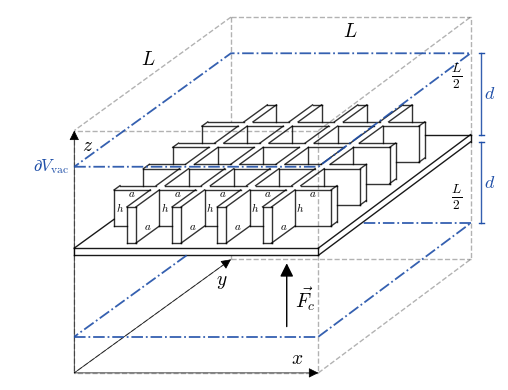
\includegraphics[width=0.42\textwidth]{honeycomb_box_L_d.png}
\caption{}{\centering{\textbf{Рис.2.} Грани «коробочки» \(\partial V_{\mathrm{vac}}\) при \(z=\pm d\).}}
\end{center}
\label{fig:honeycomb_box_L_d}
\end{figure}

\textbf{«Коробочка».} Охватим пластину замкнутой поверхностью \(\partial V_{\mathrm{vac}}\) с
гранями \(z=+d\) и \(z=-d'\) (\(0<d\le l\), \(0<d'\le L-l\)) на всё сечение \(L\times L\) (рис.~2);
боковые грани лежат на стенках куба, где \(T_{zx}=T_{zy}=0\). Тогда
\[
\begin{aligned}
F_z&=\oint_{\partial V_{\mathrm{vac}}}\langle T_{zz}\rangle\,da
=\left[\langle T_{zz}\rangle(d)-\langle T_{zz}\rangle(-d')\right]L^2\\
&=(p_{\text{big}}-p_{\text{cell}})\,L^2 .
\end{aligned}
\]
По доказанной независимости от \(z\) результат не зависит от \(d\), \(d'\). При \(d,d'\to0\) это
сумма двух скачков на гранях пластины --- сила приложена к поверхностям металла; при \(d=l\),
\(d'=L-l\) грани подходят к вспомогательным стенкам куба (при \(l=L/2\) --- грани
\(z=\pm L/2\)), понимаемым как предел изнутри полостей. На сотовой стороне грань пересекает
стенки ячеек; при нулевой толщине стенок они вклада в интеграл не дают. \(F_z>0\) (толчок в
сторону ячеек) при \(p_{\text{big}}>p_{\text{cell}}\).

Поток через \(\partial V_{\mathrm{vac}}\) --- это поток импульса \emph{поля} через чисто вакуумную
границу, а не сила, приложенная непосредственно к веществу. Он отличен от нуля лишь потому, что
спектр мод, а значит и \(\langle T_{zz}\rangle\), различен на сотовой и на гладкой стороне.

\vspace{\myvspacebeforesubsection}
\subsection*{\centering{\fontencoding{T2A}\fontfamily{ptm}{\selectfont ПОЧЕМУ СТАНДАРТНЫЙ БАЛАНС ИМПУЛЬСА ЭТОГО НЕ ВИДИТ}}}
\vspace{\myvspaceaftersubsection}


Стандартное уравнение баланса импульса электродинамики сплошных сред (Тамм, \S\,105
\cite{Tamm1957}) имеет вид

\end{multicols}
\[
\nabla\cdot\mathbf{T} = \frac{\partial\mathbf{g}}{\partial t} + \mathbf{f}_{\mathrm{vol}},
\qquad
\mathbf{g} = \frac{1}{c^2}\mathbf{S} = \frac{1}{4\pi c}[\mathbf{E}\times\mathbf{H}],
\]
\begin{multicols}{2}

где \(\mathbf{g}\) --- плотность импульса поля, \(\mathbf{f}_{\mathrm{vol}}\) --- плотность
объёмной пондеромоторной силы. Для вакуумных флуктуаций статической сотовой системы
\(\langle\mathbf{S}\rangle=0\), следовательно, \(\langle\partial\mathbf{g}/\partial t\rangle=0\).
Если отождествить импульс поля с \(\mathbf g\), то при \(\langle\mathbf S\rangle=0\) нет и
переноса импульса --- и однотельная сила кажется невозможной.

Переход от объёмных сил к натяжениям опирается на теорему Гаусса, которую Тамм применяет
(\S\,33, ф.~33.7) при явном условии \emph{непрерывности} компонент тензора внутри объёма;
поверхности разрыва там исключены, а позже (\S\,34, ф.~34.8) рассматриваются лишь их
поверхностные \emph{заряды}. Но, как показано выше, граница вакуум--металл может не нести
поверхностного заряда и всё же давать конечный скачок тензора натяжений. Этот случай не
рассмотрен ни в \S\,33, ни где-либо ещё в книге Тамма, включая \S\,105. Для объёма \(V\),
содержащего внутренние поверхности разрыва \(S_j\), теорему Гаусса нужно записывать в виде

\end{multicols}
\[
\int_V \frac{\partial T_{ik}}{\partial x_k}\,dV
= \oint_{\partial V_{\mathrm{ext}}} T_{ik}\,n_k\,dS
\;-\; \sum_j \int_{S_j} [\![\,T_{ik}\,]\!]\,n_k\,dS_j ,
\]
\begin{multicols}{2}

где \([\![\cdot]\!]\) --- скачок величины при переходе через \(S_j\). Привычное отождествление
импульса поля с \(\mathbf{g}=\mathbf{S}/c^2\) сохраняет лишь внешний поверхностный интеграл и
теряет скачковые члены. Для сотовой пластины именно они и составляют всю силу: сумма двух
скачков на гранях пластины равна потоку через «коробочку».

Два замечания делают интерпретацию однозначной. Во-первых, как уже сказано, не сохраняется
импульс \emph{поля} (и поглощающей его пластины), а не полный импульс замкнутой лабораторной
системы. Во-вторых, перенормированное вакуумное натяжение \(\langle T_{\mu\nu}\rangle\) является
физически измеримой величиной --- это и есть сам эффект Казимира, --- поэтому скачковые члены
не требуют предположения о материальном эфире: их значение задаётся тем же
\(\langle T_{\mu\nu}\rangle\), которое подтверждено экспериментально для симметричной
конфигурации.

\vspace{\myvspacebeforesubsection}
\subsection*{\centering{\fontencoding{T2A}\fontfamily{ptm}{\selectfont ПРОВЕРКИ И ОЦЕНКИ}}}
\vspace{\myvspaceaftersubsection}


\textbf{Две пластины Казимира.} Пластины при \(z=0\) и \(z=a\), внешние полости до \(z=\pm L/2\).
В зазоре \(k_z=\pi n/a\), поперечный спектр непрерывен; на единицу площади (две поляризации)
\[
p_{\text{in}}=\frac{\hbar c}{a}\sum_{n\ge1}\int\frac{d^2k_\parallel}{(2\pi)^2}\frac{k_z^2}{k},
\]
а снаружи сумма по \(n\) заменяется на \(\frac a\pi\int dk_z\). По независимости от \(z\)
значение \(p_{\text{in}}\) одно и то же в центре зазора и у внутренней поверхности каждой
пластины, а \(p_{\text{out}}\) --- у внешней поверхности и на гранях \(z=\pm L/2\). С обрезанием
\(e^{-k/k_m}\) разность \(p_{\text{in}}-p_{\text{out}}\) равна \(-0{,}041043\), \(-0{,}041110\),
\(-0{,}041120\) в единицах \(\hbar c/a^4\) при \(k_ma=20\), \(50\), \(100\) и стремится к
\(-\pi^2/240=-0{,}041123\). Знак означает притяжение; с плотностью энергии Казимира
\(u=-\pi^2\hbar c/720a^4\) это соотношение \(p=3u\) \cite{BrownMaclay1969}.

\textbf{Тензорная сумма для сот.} Для сотовой пластины тензорная сумма \(\sum k_z^2/k\) с
регулятором \(f=1/(1+k^4/k_m^4)\) вычислена тем же двумерным суммированием, что и энергетическая
в \cite{Drozdov2024}. Обозначим \(D_E\) и \(D_T\) энергетическую и тензорную разности
«сумма минус интеграл». При малых \(ak_m\) они различаются даже знаком (член с \(f'\)), но при
\(ak_m=9\) и \(14\) получено \(D_T+D_E=1\cdot10^{-4}\) и \(4\cdot10^{-6}\) соответственно при
\(|D_E|\approx0{,}012\): в пределе \(ak_m\to\infty\) тензорный и гамильтонов выводы дают одну и
ту же силу, \(|F/S|=\delta(E/V)\), в согласии с буст-аргументом.

\textbf{Оценка тяги.} При \(\hbar c\,\pi/a^4=0{,}9932/a_\mu^4\)~дин/см\(^2\) (\(a_\mu\) --- сторона
ячейки в микронах) значение \(R=0{,}0138\) из таблицы~1 работы \cite{Drozdov2024} даёт для
золотых сот с \(a\approx2\)~мкм \(F/S\approx8{,}55\)~дин/м\(^2\)
\(=8{,}55\times10^{-5}\)~Н/м\(^2\). Повторный расчёт той же величины с явным контролем сходимости
по области суммирования воспроизводит таблицу~1 при \(ak_m\lesssim3\), но при \(ak_m\gtrsim4\)
даёт меньшие по модулю значения; предел \(|R|\approx0{,}0121\) соответствует
\(F/S\approx7{,}5\)~дин/м\(^2\). Порядок величины и вывод о практической применимости для
коррекции орбит спутников от этого не меняются.

\vspace{\myvspacebeforesubsection}
\subsection*{\centering{\fontencoding{T2A}\fontfamily{ptm}{\selectfont ОГРАНИЧЕНИЯ}}}
\vspace{\myvspaceaftersubsection}


(а) \textit{Высота ячеек.} Расчёт предполагает, что стенки ячеек доходят до грани куба и ячейка
является замкнутым резонатором. Для реальных ячеек высотой \(h\ll L\) ячейка открыта в большую
полость, моды не разделяются, и этот расчёт такой случай не описывает.

(б) \textit{Идеальный проводник.} Скачок есть свойство идеального проводника. В реальном металле
\(T_{zz}\) спадает до нуля на толщине скин-слоя, а интеграл силы по слою равен скачку, пока ток в
металле согласован с полем: \(\mathbf j=\frac c{4\pi}\nabla\times\mathbf H\).

(в) \textit{Толщина стенок.} Стенки ячеек конечной толщины не несут \(z\)-силы (\(T_{zx}=0\) на
них), но уменьшают долю площади пластины, занятую полостями.

(г) \textit{Регуляризация.} Какая из двух регуляризованных величин --- энергетическая или
тензорная --- физична при конечном \(ak_m\), в модели идеального проводника с модовым обрезанием
решить нельзя; для этого нужна реальная \(\varepsilon(\omega)\), как в методе Дзялошинского,
Лифшица и Питаевского \cite{DLP1961}, где натяжение в вакуумном зазоре находится из функции
Грина поля. Для ячейки сот для этого нужна функция Грина прямоугольного волновода; это оставлено
для дальнейшей работы.

(д) \textit{Квантовое среднее.} Равенство электрической и магнитной частей энергии моды в
основном состоянии использовано как стандартный результат для осциллятора и здесь не выводится.

\vspace{\myvspacebeforesubsection}
\subsection*{\centering{\fontencoding{T2A}\fontfamily{ptm}{\selectfont ЗАКЛЮЧЕНИЕ}}}
\vspace{\myvspaceaftersubsection}


Сотовый двигатель Казимира является примером физической системы, в которой теорема Нётер
непосредственно объясняет происхождение макроскопической силы: \textbf{отсутствие
пространственной однородности приводит к несохранению импульса поля}, а следовательно, к
появлению тяги. Независимый расчёт через тензор натяжений Максвелла, построенный из полей мод,
воспроизводит ту же силу --- помодово тождественно и после регуляризации в пределе
\(ak_m\to\infty\), --- и при этом исправляет ошибку в приложении~B работы \cite{Drozdov2024}.
Тензорный расчёт показывает, что сила приложена к поверхностям металла в виде скачка
\(\langle T_{zz}\rangle\), а стандартный баланс импульса \S\,105 Тамма, сведённый к
\(\mathbf g=\mathbf S/c^2\), этих скачковых членов не содержит. Полный импульс системы
\emph{пластина\,+\,поле\,+\,опора} сохраняется. Экспериментальная проверка эффекта могла бы
подтвердить связь между геометрией граничных условий, симметрией и динамикой квантового вакуума.

\vspace{\myvspacebeforesubsection}
\subsection*{\centering{\fontencoding{T2A}\fontfamily{ptm}{\selectfont ПРИЛОЖЕНИЕ А. ПОЛЯ МОД}}}
\vspace{\myvspaceaftersubsection}


Поля TM-моды (\(H_z=0\), \(n_x,n_y\ge1\), \(n_z\ge0\)):
\end{multicols}
\[
\begin{aligned}
E_z&=A\sin k_xx\,\sin k_yy\,\cos k_zz\,\cos\omega t, &
H_z&=0,\\
E_x&=-A\frac{k_xk_z}{K^2}\cos k_xx\,\sin k_yy\,\sin k_zz\,\cos\omega t, &
H_x&=-A\frac{k\,k_y}{K^2}\sin k_xx\,\cos k_yy\,\cos k_zz\,\sin\omega t,\\
E_y&=-A\frac{k_yk_z}{K^2}\sin k_xx\,\cos k_yy\,\sin k_zz\,\cos\omega t, &
H_y&=A\frac{k\,k_x}{K^2}\cos k_xx\,\sin k_yy\,\cos k_zz\,\sin\omega t.
\end{aligned}
\]
Поля TE-моды (\(E_z=0\), \(n_z\ge1\), \((n_x,n_y)\ne(0,0)\)):
\[
\begin{aligned}
H_z&=A\cos k_xx\,\cos k_yy\,\sin k_zz\,\cos\omega t, &
E_z&=0,\\
H_x&=-A\frac{k_xk_z}{K^2}\sin k_xx\,\cos k_yy\,\cos k_zz\,\cos\omega t, &
E_x&=-A\frac{k\,k_y}{K^2}\cos k_xx\,\sin k_yy\,\sin k_zz\,\sin\omega t,\\
H_y&=-A\frac{k_yk_z}{K^2}\cos k_xx\,\sin k_yy\,\cos k_zz\,\cos\omega t, &
E_y&=A\frac{k\,k_x}{K^2}\sin k_xx\,\cos k_yy\,\sin k_zz\,\sin\omega t.
\end{aligned}
\]
\begin{multicols}{2}

Подстановкой проверяется, что \(\nabla\cdot\mathbf E=\nabla\cdot\mathbf H=0\),
\(\nabla\times\mathbf E=-\frac1c\partial_t\mathbf H\), \(\nabla\times\mathbf H=\frac1c\partial_t\mathbf E\)
при \(\omega=ck\), и что выполнены граничные условия идеального проводника: касательное
\(\mathbf E\) и нормальное \(\mathbf H\) обращаются в нуль на всех шести гранях (на \(x=0,a\):
\(E_y=E_z=0\), \(H_x=0\); на \(y=0,b\): \(E_x=E_z=0\), \(H_y=0\); на \(z=0,h\): \(E_x=E_y=0\),
\(H_z=0\)). Эти соотношения проверены символьно и численно для моды \((2,1,3)\) при
\(a:b:h=1:1{,}3:2{,}7\).

Для TE-моды усреднение по сечению и периоду даёт
\(\langle H_z^2\rangle=\frac{A^2}{8}\sin^2k_zz\),
\(\langle H_x^2+H_y^2\rangle=\frac{A^2}{8}\frac{k_z^2}{K^2}\cos^2k_zz\),
\(\langle E_x^2+E_y^2\rangle=\frac{A^2}{8}\frac{k^2}{K^2}\sin^2k_zz\), откуда
\(8\pi\langle T_{zz}\rangle=-\frac{A^2}{8}\frac{k_z^2}{K^2}\) и \(p=\overline w\,k_z^2/k^2\).

\end{multicols}

\newpage

\fontencoding{T1}\fontfamily{ptm}\selectfont

\section*{\centering {\fontencoding{T1}\fontfamily{ptm}{\selectfont \uppercase{\mytitleen}}}}

\centerline{\Large{\mynameen \,\orcidlink{\myorcidlink} }}
\vspace{3mm}
\centerline{\textit{\myworkplaceen}}
\centerline{\textit{E-mail: \href{mailto:\myemail}{\myemail}}}

\vspace{3mm}
\centerline{\myreceiveden}
\centerline{\myaccepteden}

\vspace{3.5mm}

The Casimir honeycomb drive \cite{Drozdov2024} --- a perfectly conducting plate with a
nanoscale honeycomb structure on one side --- is examined from the standpoint of symmetries.
Because the vacuum modes on the two sides of the plate differ, the system is not invariant under
translations along the normal: the vacuum Hamiltonian depends explicitly on the coordinate \(l\),
and by Noether's theorem the field momentum along this axis is not conserved. The thrust equals
\(\partial\langle H\rangle/\partial l\). The same force is then computed independently, from the
Maxwell stress tensor built out of the fields of the cavity eigenmodes. Mode by mode the two
derivations coincide identically (Hellmann--Feynman theorem); after regularization they coincide
in the limit \(ak_m\to\infty\). Along the way an error in Appendix~B of \cite{Drozdov2024} is
found and corrected: for TM modes the ratio of pressure to energy density is \(k_z^2/k^2\), not
unity. The stress-tensor calculation shows where the force acts: it is the jump of
\(\langle T_{zz}\rangle\) at the metal surface, which is why the momentum flux through any closed
vacuum surface enclosing the plate is independent of the position of its faces. Finally, it is
shown that the standard momentum balance (Tamm, \S\,105) with \(\langle\mathbf S\rangle=0\) loses
exactly these jump terms. What is not conserved is the momentum of the field (and of the plate);
the total momentum of the system \emph{plate\,+\,field\,+\,support} is conserved.

\vspace{3mm}

\noindent
\textbf{\textit{Keywords:}} \textit{Noether's theorem, Casimir effect, quantum vacuum, momentum non-conservation, Maxwell stress tensor, nanohoneycomb, Casimir thrust}

\fontencoding{T2A}\fontfamily{ptm}\selectfont

\begin{thebibliography}{9}
\bibitem{Drozdov2024}
А. Дроздов, \textit{Сотовый двигатель Казимира: о силе, действующей на идеально проводящие соты на пластине}, Вестник Харьковского национального университета имени В.~Н.~Каразина, серия «Физика», вып. 41, 28--41 (2024). \url{https://doi.org/10.26565/2222-5617-2024-41-04}
\bibitem{Noether1918}
E. Noether, \textit{Invariante Variationsprobleme}, Nachr. d. König. Gesellsch. d. Wiss. zu Göttingen, Math-phys. Klasse, 235–257 (1918).
\bibitem{Casimir1948}
H. B. G. Casimir, \textit{On the attraction between two perfectly conducting plates}, Proc. K. Ned. Akad. Wet. B \textbf{51}, 793 (1948).
\bibitem{Tamm1957}
И. Е. Тамм, \textit{Основы теории электричества} (\S\,105, тензор натяжений Максвелла и баланс импульса электромагнитного поля), Наука, Москва.
\bibitem{Feynman1939}
R. P. Feynman, \textit{Forces in molecules}, Phys. Rev. \textbf{56}, 340 (1939).
\bibitem{BrownMaclay1969}
L. S. Brown, G. J. Maclay, \textit{Vacuum stress between conducting plates: an image solution}, Phys. Rev. \textbf{184}, 1272 (1969).
\bibitem{Weyl1912}
H. Weyl, \textit{Das asymptotische Verteilungsgesetz der Eigenwerte linearer partieller Differentialgleichungen}, Math. Ann. \textbf{71}, 441 (1912).
\bibitem{DLP1961}
И. Е. Дзялошинский, Е. М. Лифшиц, Л. П. Питаевский, \textit{Общая теория ван-дер-ваальсовых сил}, УФН \textbf{73}, 381 (1961).
\bibitem{VerifNotebook}
А. Дроздов, \textit{Проверочные расчёты к статье «Теорема Нётер и сотовый двигатель Казимира»}, Jupyter-ноутбук (SageMath 9.6), GitHub (2026). \url{https://github.com/daju1/articles/blob/master/casimir_noether/noether_casimir_verification.ipynb}
\end{thebibliography}

\end{document}
